\section{Experimental Study}
\label{sec-exp}

We evaluate the filtered search along four research questions.
\begin{itemize}
\item \textbf{[RQ1] Order}: how much of a term's neighborhood does a sorted order of an
  ontology hold? (Table~\ref{tab-order}, Section~\ref{sec-order}.)
\item \textbf{[RQ2] Filtered search}: what do the strategies return and cost, against
  FAISS filtering with ID selectors?
\item \textbf{[RQ3] The rule}: is the class filter correlated with the vectors, does testing
  it per row beat resolving it, and where is the crossover?
\item \textbf{[RQ4] The indexes}: what do IVF with lists in the triple tree and HNSW cost
  against FAISS and hnswlib, and does the design scale to 218,723 terms?
\end{itemize}

\stitle{Setup}.
The ontologies are the Gene Ontology~\cite{ashburner2000} (38,092 terms, release
2026-07-26 without obsolete terms), the Human Phenotype Ontology~\cite{kohler2021}
(19,894), Uberon~\cite{mungall2012} (15,047), and ChEBI~\cite{hastings2016} (218,723),
each with the \texttt{is\_a} edges as the hierarchy and the term names embedded by
\texttt{all-MiniLM-L6-v2}~\cite{reimers2019} into 384 dimensions on a CPU.
For each ontology and each of five sizes of $|\desc(c)|$ ($\le$10, 11--100, 101--1,000,
1,001--5,000, $>$5,000) we draw up to 20 classes that have subclasses, and for each class
three queries: a stored term inside the class, one outside it, and the embedding of a
synonym of a stored member (5,000 synonyms sampled per ontology), which is not a stored
vector.
Answers are scored against exact search over the class's members, with the query term
excluded; there are 958 queries per strategy.
OntoDB uses IVF with $\nu=2.6\sqrt N$ lists and $\rho=16$, HNSW with $M{=}16$,
construction beam 200, and $\ef{=}64$, and the auto rule with $\theta=4{,}096$; FAISS
1.15.1 uses \texttt{IndexFlatIP}, \texttt{IndexIVFFlat} (same $\nu$, nprobe 16), and
\texttt{IndexHNSWFlat} (same $M$, efSearch 64), each searched with an
\texttt{IDSelectorBitmap} of the class's members; hnswlib 0.8.0 appears in the unfiltered
comparison.
The members of a class for FAISS come from a descendant table built outside the timer,
which favors FAISS.
Every time is the mean of three runs after one warm-up, on one thread of an Apple M2 Pro
with 16\,GiB; FAISS is called once per query from Python, and its call overhead (about
10\,$\mu$s) is included.

\subsection{RQ2: Filtered Search}

\begin{table*}[t]
\caption{Ten nearest terms under a class: recall@10 / microseconds per query, by number of classes below $c$ and by query kind, pooled over 4 ontologies. FAISS runs each query with an ID selector of the class's members (their lookup is not timed). Bold marks the fastest strategy with recall at least 0.99; blue marks \sys{}.}
\label{tab-filtered}
\small
\begin{tabular}{@{}llccccccc@{}}
\toprule
Below $c$ & query & DuckDB join & FAISS exact & FAISS IVF & FAISS HNSW & pre-filter & masked HNSW & auto \\
\midrule
$\le$10 & inside $c$ & 1.00 / 718 & 1.00 / 71 & 0.79 / 29 & 0.87 / 50 & \cellcolor{ours}\textbf{1.00 / 2.1} & 1.00 / 42.1\,k & 1.00 / 2.2 \\
11--100 &  & 1.00 / 811 & 1.00 / 72 & 0.82 / 30 & 0.85 / 49 & \cellcolor{ours}\textbf{1.00 / 7.9} & 1.00 / 37.4\,k & 1.00 / 8.1 \\
101--1,000 &  & 1.00 / 1.2\,k & 1.00 / 90 & 0.89 / 35 & 0.91 / 50 & \cellcolor{ours}\textbf{1.00 / 47} & 1.00 / 5.9\,k & 1.00 / 49 \\
1,001--5,000 &  & 1.00 / 2.6\,k & \textbf{1.00 / 213} & 0.93 / 46 & 0.98 / 47 & 1.00 / 244 & 1.00 / 1.2\,k & 1.00 / 396 \\
$>$5,000 &  & 1.00 / 28.6\,k & 1.00 / 2.0\,k & 0.93 / 81 & 0.98 / 56 & 1.00 / 4.9\,k & 1.00 / 506 & \cellcolor{ours}\textbf{1.00 / 456} \\
\midrule
$\le$10 & outside $c$ & 1.00 / 708 & 1.00 / 69 & 0.05 / 29 & 0.02 / 51 & \cellcolor{ours}\textbf{1.00 / 2.1} & 1.00 / 42.2\,k & 1.00 / 2.2 \\
11--100 &  & 1.00 / 802 & 1.00 / 71 & 0.06 / 29 & 0.04 / 49 & \cellcolor{ours}\textbf{1.00 / 7.8} & 1.00 / 38.8\,k & 1.00 / 8.3 \\
101--1,000 &  & 1.00 / 1.1\,k & 1.00 / 88 & 0.23 / 29 & 0.24 / 50 & \cellcolor{ours}\textbf{1.00 / 47} & 1.00 / 18.2\,k & 1.00 / 51 \\
1,001--5,000 &  & 1.00 / 2.6\,k & \textbf{1.00 / 205} & 0.40 / 33 & 0.39 / 49 & 1.00 / 245 & 1.00 / 9.3\,k & 1.00 / 652 \\
$>$5,000 &  & 1.00 / 27.4\,k & 1.00 / 2.0\,k & 0.58 / 61 & 0.73 / 62 & 1.00 / 5.0\,k & 0.99 / 1.9\,k & \cellcolor{ours}\textbf{0.99 / 1.9\,k} \\
\midrule
$\le$10 & synonym of a member & 1.00 / 708 & 1.00 / 49 & 0.74 / 25 & 0.76 / 48 & \cellcolor{ours}\textbf{1.00 / 2.2} & 1.00 / 25.3\,k & 1.00 / 2.3 \\
11--100 &  & 1.00 / 808 & 1.00 / 56 & 0.74 / 27 & 0.74 / 47 & \cellcolor{ours}\textbf{1.00 / 7.7} & 1.00 / 27.1\,k & 1.00 / 8.0 \\
101--1,000 &  & 1.00 / 1.1\,k & 1.00 / 87 & 0.82 / 33 & 0.88 / 51 & \cellcolor{ours}\textbf{1.00 / 47} & 1.00 / 8.9\,k & 1.00 / 50 \\
1,001--5,000 &  & 1.00 / 2.6\,k & \textbf{1.00 / 203} & 0.79 / 42 & 0.90 / 50 & 1.00 / 246 & 1.00 / 3.7\,k & 1.00 / 257 \\
$>$5,000 &  & 1.00 / 28.1\,k & \textbf{1.00 / 2.0\,k} & 0.88 / 75 & 0.91 / 59 & 1.00 / 5.1\,k & 0.98 / 615 & 0.98 / 596 \\
\bottomrule
\end{tabular}
\end{table*}


\stitle{Approximate indexes lose recall silently}.
Table~\ref{tab-filtered} and Figure~\ref{fig-recall} give the result.
Over the 958 queries FAISS's IVF and HNSW with an ID selector return recall 0.61 and 0.64,
and 59\% and 52\% of their queries are below 0.99.
The loss is worst where the filter is most selective and the query is far from it: for
a query outside a class of at most ten members they return 0.05 and 0.02.
A larger budget does not repair it (Table~\ref{tab-wide}): with half of all lists probed,
IVF reaches 0.52 for those queries at three times the time, and HNSW with a beam of 1,024
reaches 0.20 at 26 times the time, because the walk and the probed lists are the ones
near the query, where no member lives.
Over all queries the wide IVF reaches recall 0.91 in 204\,$\mu$s on average, the same time as
the rule, and 19\% of its queries are still below 0.99; the wide HNSW reaches 0.81 in 1.2\,ms.

\begin{figure}[t]
\centering
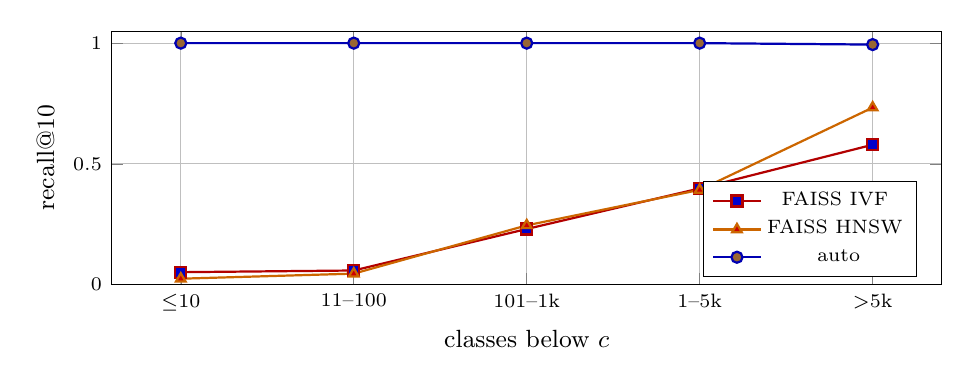
\begin{tikzpicture}
\begin{axis}[width=\columnwidth,height=4.8cm,symbolic x coords={<=10,11-100,101-1000,1001-5000,>5000},xtick=data,xticklabels={$\le$10,11--100,101--1k,1--5k,$>$5k},xlabel={classes below $c$},ylabel={recall@10},ymin=0,ymax=1.05,grid=both,legend pos=south east,legend style={font=\scriptsize},tick label style={font=\scriptsize},label style={font=\small}]
\addplot+[mark=square*,color=red!70!black,thick] coordinates {(<=10,0.051) (11-100,0.058) (101-1000,0.230) (1001-5000,0.398) (>5000,0.579)};
\addlegendentry{FAISS IVF}
\addplot+[mark=triangle*,color=orange!80!black,thick] coordinates {(<=10,0.024) (11-100,0.045) (101-1000,0.245) (1001-5000,0.392) (>5000,0.733)};
\addlegendentry{FAISS HNSW}
\addplot+[mark=*,color=blue!70!black,thick] coordinates {(<=10,1.000) (11-100,1.000) (101-1000,1.000) (1001-5000,1.000) (>5000,0.994)};
\addlegendentry{\sys{} auto}
\end{axis}
\end{tikzpicture}

\caption{Recall@10 for queries outside the class, by number of classes below it (pooled over the four ontologies).}
\label{fig-recall}
\end{figure}

\begin{table}[t]
\caption{FAISS with an ID selector at its default budget and at a much larger one (half of all IVF lists; HNSW beam 1,024): recall@10 / microseconds, queries outside the class, pooled.}
\label{tab-wide}
\small
\resizebox{\columnwidth}{!}{%
\begin{tabular}{@{}lrrrr@{}}
\toprule
Below $c$ & IVF & IVF, half the lists & HNSW & HNSW, beam 1,024 \\
\midrule
$\le$10 & 0.05 / 29 & 0.52 / 86 & 0.02 / 51 & 0.20 / 1.3\,k \\
11--100 & 0.06 / 29 & 0.68 / 88 & 0.04 / 49 & 0.35 / 1.2\,k \\
101--1,000 & 0.23 / 29 & 0.89 / 99 & 0.24 / 50 & 0.66 / 1.2\,k \\
1,001--5,000 & 0.40 / 33 & 0.97 / 160 & 0.39 / 49 & 0.78 / 1.2\,k \\
$>$5,000 & 0.58 / 61 & 0.99 / 1.1\,k & 0.73 / 62 & 0.95 / 1.5\,k \\
\bottomrule
\end{tabular}}
\end{table}


\stitle{Why}.
Table~\ref{tab-mechanism} shows the mechanism for IVF.
The lists an IVF index probes are the ones nearest the query, and the members of a small
class are somewhere else: for a query outside a class of at most ten members (four on
average), the 16 probed lists hold 0.2 of them, and outside a class of 11 to 100 (31 on
average) 1.1, where the answer needs ten.
For a query inside, they hold 3.5 of four and 19 of 31.
An index that cannot find allowed rows in the region it searches returns what it has,
and a filtered HNSW walk behaves the same way: it fills its beam with near nodes that are
not members.

\begin{table}[t]
\caption{Why an ID-selector IVF loses recall: the members of the class that lie in the 16 lists it probes, against the ten the answer needs (mean over the queries, pooled over the four ontologies).}
\label{tab-mechanism}
\small
\begin{tabular}{@{}lrrr@{}}
\toprule
Below $c$ & members & in probed lists, inside & outside \\
\midrule
$\le$10 & 4 & 3.5 & 0.2 \\
11--100 & 31 & 19.2 & 1.1 \\
101--1,000 & 308 & 120.8 & 12.6 \\
1,001--5,000 & 1,856 & 397.7 & 48.1 \\
$>$5,000 & 36,431 & 1,139.9 & 585.4 \\
\bottomrule
\end{tabular}
\end{table}


\begin{figure}[t]
\centering
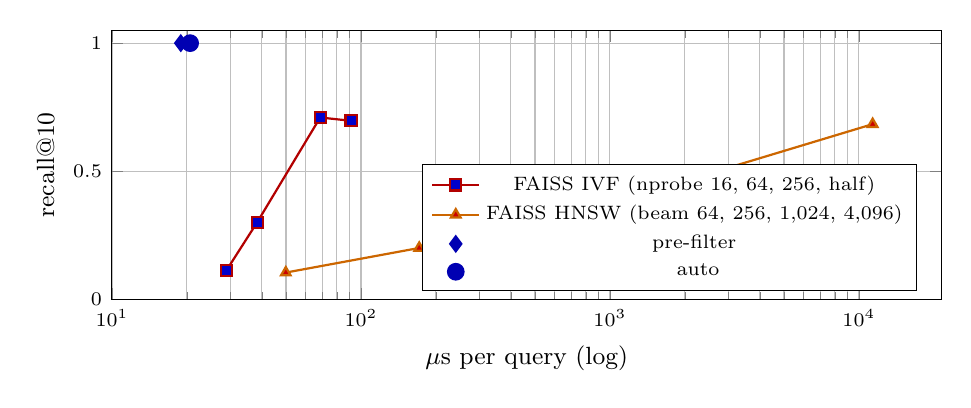
\begin{tikzpicture}
\begin{axis}[width=\columnwidth,height=5.0cm,xmode=log,xlabel={$\mu$s per query (log)},ylabel={recall@10},ymin=0,ymax=1.05,grid=both,legend pos=south east,legend style={font=\scriptsize},tick label style={font=\scriptsize},label style={font=\small}]
\addplot+[mark=square*,color=red!70!black,thick] coordinates {(28.8,0.113) (38.3,0.301) (68.6,0.710) (91.3,0.697)};
\addlegendentry{FAISS IVF (nprobe 16, 64, 256, half)}
\addplot+[mark=triangle*,color=orange!80!black,thick] coordinates {(49.9,0.105) (171.4,0.201) (1231.3,0.401) (11354.3,0.684)};
\addlegendentry{FAISS HNSW (beam 64, 256, 1,024, 4,096)}
\addplot[only marks,mark=diamond*,mark size=3pt,color=blue!70!black] coordinates {(18.9,1.000)};
\addlegendentry{pre-filter}
\addplot[only marks,mark=*,mark size=3pt,color=blue!70!black] coordinates {(20.6,1.000)};
\addlegendentry{\sys{} auto}
\end{axis}
\end{tikzpicture}

\caption{What more search effort buys FAISS on queries outside classes of up to 1,000 members: recall@10 against mean microseconds, pooled over the ontologies, for four IVF and four HNSW budgets, and the two strategies of the rule.}
\label{fig-budget}
\end{figure}

\stitle{A relational baseline}.
DuckDB with a closure table of (class, member) pairs and one SQL statement per query, which
joins the class's members to their vectors and orders by inner product, is exact like
pre-filtering and has nothing to lose recall: its mean is 4.0\,ms and its median 0.97\,ms,
0.7\,ms for classes of at most ten members, where the rule takes 2.1\,$\mu$s, and 28\,ms
for classes above 5,000.
The hierarchy is the same in both; the difference is that a range scan of a B+ tree that
already holds the labels replaces a join, and a dot-product loop replaces a query plan.
\begin{figure}[t]
\centering
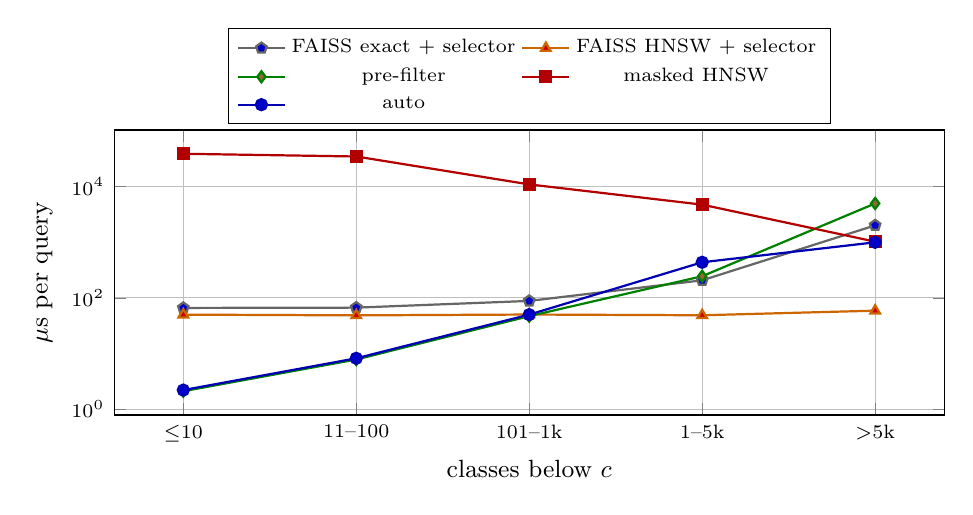
\begin{tikzpicture}
\begin{axis}[width=\columnwidth,height=5.2cm,ymode=log,symbolic x coords={<=10,11-100,101-1000,1001-5000,>5000},xtick=data,xticklabels={$\le$10,11--100,101--1k,1--5k,$>$5k},xlabel={classes below $c$},ylabel={$\mu$s per query},grid=both,legend style={font=\scriptsize,at={(0.5,1.02)},anchor=south,legend columns=2},tick label style={font=\scriptsize},label style={font=\small}]
\addplot+[mark=pentagon*,color=black!60,thick] coordinates {(<=10,66.0) (11-100,66.8) (101-1000,88.2) (1001-5000,207.0) (>5000,2011.9)};
\addlegendentry{FAISS exact + selector}
\addplot+[mark=triangle*,color=orange!80!black,thick] coordinates {(<=10,50.0) (11-100,48.5) (101-1000,50.2) (1001-5000,48.7) (>5000,58.9)};
\addlegendentry{FAISS HNSW + selector}
\addplot+[mark=diamond*,color=green!50!black,thick] coordinates {(<=10,2.1) (11-100,7.8) (101-1000,47.0) (1001-5000,244.9) (>5000,4987.1)};
\addlegendentry{pre-filter}
\addplot+[mark=square*,color=red!70!black,thick] coordinates {(<=10,38996.8) (11-100,34846.6) (101-1000,10971.5) (1001-5000,4747.7) (>5000,1025.3)};
\addlegendentry{masked HNSW}
\addplot+[mark=*,color=blue!70!black,thick] coordinates {(<=10,2.2) (11-100,8.2) (101-1000,50.0) (1001-5000,436.9) (>5000,997.7)};
\addlegendentry{auto}
\end{axis}
\end{tikzpicture}

\caption{Mean microseconds per query by number of classes below $c$, pooled over the ontologies and query kinds (log scale).}
\label{fig-latency}
\end{figure}

\stitle{Interval filtering is exact and fast where it matters}.
The auto rule returns recall 0.999, and none of its 958 queries is below 0.99; its median
is 26\,$\mu$s and its mean 206\,$\mu$s.
An exact FAISS scan with the same selector has median 60\,$\mu$s and mean 300\,$\mu$s, so
the rule is 2.3 times faster at the median and 1.5 times on average, while the approximate
indexes, which are 4 to 6 times faster than the rule on average (50 and 36\,$\mu$s), are
wrong more often than right.
The gain is largest for small classes: with at most ten members, pre-filtering takes
2.1\,$\mu$s, 33 times less than the 70\,$\mu$s of the FAISS scan, which must test a
bitmap against all $N$ rows.
From 1,001 to 5,000 members the FAISS scan is faster than pre-filtering (214 against
244\,$\mu$s inside) and than the rule (396\,$\mu$s inside, 652 outside);
above 5,000 members the rule's masked HNSW beats the exact scan for queries inside the
class (456 against 2,000\,$\mu$s) and matches it for queries outside (1.9 against 2.0\,ms).
Synonym queries, whose vectors are not stored, behave like inside queries.

\subsection{RQ3: The Rule}

Table~\ref{tab-correlation} shows the correlation: for a query inside a class of 101 to
1,000 members, 31\% of the unfiltered top 100 lie under the class, where an independent
filter would pass 1.2\% of the terms, and for a query outside it 1\%; for the largest
classes 59\% inside against 33\% expected, and 24\% outside.
The independence estimate $k/f(c)$ of the candidates a post-filter needs is therefore too
high inside and too low outside, and the post-filtering strategies show it: post-filtered
HNSW takes 34.5\,ms on average because it must widen until it finds $k$ allowed rows, and
post-filtered IVF has recall 0.61 because it stops widening too soon.

\begin{table}[t]
\caption{Masked HNSW with the filter tested per row against the class's intervals, and with the filter resolved first into a bitmap by range scans (resolving is timed): microseconds per query, pooled over the ontologies.}
\label{tab-resolve}
\small
\begin{tabular}{@{}lrrr@{}}
\toprule
Below $c$ & interval test & resolve, then bitmap & ratio \\
\midrule
$\le$10 & 42.2\,k & 41.1\,k & 1.0$\times$ \\
11--100 & 38.1\,k & 37.4\,k & 1.0$\times$ \\
101--1,000 & 12.0\,k & 11.9\,k & 1.0$\times$ \\
1,001--5,000 & 5.3\,k & 5.4\,k & 1.0$\times$ \\
$>$5,000 & 1.2\,k & 3.3\,k & 2.7$\times$ \\
\bottomrule
\end{tabular}
\end{table}


\noindent
Testing the filter per row costs the same as resolving it into a bitmap up to 5,000
members (Table~\ref{tab-resolve}) and 2.7 times less above, where resolving takes more
time than the walk it serves.
The cost model of Section~\ref{sec-filter} predicts the crossover: the mean pre-filter
cost per member is $\gamma_m=0.15\,\mu$s (median 0.11), and the masked walk over classes of
more than 5,000 members takes $\gamma_h=506\,\mu$s for queries inside, 615 for synonyms, and
1,942 for outside queries, so $\theta=\gamma_h/\gamma_m$ is about 3,400 to 13,000.

\begin{table}[t]
\caption{The auto rule at other thresholds: mean microseconds per query over every class size and query kind (all strategies return recall at least 0.99 except as noted).}
\label{tab-threshold}
\small
\begin{tabular}{@{}lrrrr@{}}
\toprule
Threshold & GO & HPO & Uberon & ChEBI \\
\midrule
256 & 609 & 246 & 301 & 6.9\,k \\
1,024 & 456 & 169 & 71 & 3.2\,k \\
4,096 & \cellcolor{ours}\textbf{111} & \cellcolor{ours}\textbf{59} & \cellcolor{ours}\textbf{41} & 533 \\
16,384 & 148 & 62 & 79 & \cellcolor{ours}\textbf{426} \\
65,536 & 180 & 114 & 79 & 567 \\
\bottomrule
\end{tabular}
\end{table}


\begin{table}[t]
\caption{A second embedding model, \texttt{all-mpnet-base-v2} (768 dimensions): recall@10 / mean microseconds over every class size and query kind, and the share of the unfiltered top 100 under the class for queries inside and outside.}
\label{tab-model}
\small
\resizebox{\columnwidth}{!}{%
\begin{tabular}{@{}lrrrrrr@{}}
\toprule
Ontology & FAISS IVF & FAISS HNSW & pre-filter & auto & top-100 under $c$, inside & outside \\
\midrule
GO & 0.64 / 51 & 0.67 / 81 & 1.00 / 279 & 1.00 / 195 & 0.30 & 0.02 \\
HPO & 0.68 / 43 & 0.71 / 77 & 1.00 / 181 & 1.00 / 94 & 0.37 & 0.05 \\
\bottomrule
\end{tabular}}
\end{table}


\noindent
Table~\ref{tab-threshold} confirms it: a threshold of 4,096 is best on the Gene Ontology,
the Human Phenotype Ontology, and Uberon, and 16,384 on ChEBI, whose walks are costlier;
256 and 1,024 are 1.7 to 7 times slower than the best, and 65,536 is 1.3 to 1.9 times
slower.
A single threshold of 4,096 is within 25\% of the best on all four.

\stitle{The number of neighbors}.
Table~\ref{tab-k} varies $k$ on the Gene Ontology: asking for one neighbor or fifty changes
the approximate indexes' recall by at most 0.1 (0.70 to 0.55 for IVF), and the rule stays
exact, at a mean of 107 to 115\,$\mu$s.

\begin{table}[t]
\caption{The number of neighbors asked for, on the Gene Ontology: recall / mean microseconds over every class size and query kind.}
\label{tab-k}
\small
\begin{tabular}{@{}lrrrr@{}}
\toprule
$k$ & FAISS IVF & FAISS HNSW & pre-filter & auto \\
\midrule
1 & 0.70 / 31 & 0.75 / 46 & 1.00 / 173 & 1.00 / 107 \\
10 & 0.63 / 31 & 0.67 / 47 & 1.00 / 178 & 1.00 / 110 \\
50 & 0.55 / 33 & 0.56 / 49 & 1.00 / 182 & 1.00 / 115 \\
\bottomrule
\end{tabular}
\end{table}


\stitle{Another embedding model}.
Table~\ref{tab-model} repeats the study on the Gene Ontology and the Human Phenotype
Ontology with \texttt{all-mpnet-base-v2}, a larger model with 768 dimensions, and the picture
holds: FAISS's IVF and HNSW return recall 0.64 to 0.71, the rule returns 1.00, and the
correlation is as strong (0.30 and 0.37 of the unfiltered top 100 under the class for inside
queries, 0.02 and 0.05 for outside).

\stitle{Threats to validity}.
The members FAISS filters with come from a table built outside the timer, which favors it;
FAISS and DuckDB are called from Python, whose per-call overhead (about 10\,$\mu$s) matters
for the 2\,$\mu$s queries; each index is built once, so HNSW's randomness is one draw;
the ontologies are four of the OBO Foundry's, with names embedded by two sentence models,
and the queries are sampled by class size, not by use.
The comparison with FAISS's approximate indexes is one of default-style settings and of a
wide budget, not of tuned ones.

\subsection{RQ4: The Indexes}

\begin{table*}[t]
\caption{Unfiltered ten-nearest-neighbor search, 1,000 queries: recall@10 / microseconds per query. FAISS is called once per query from Python, like \sys{} (its call overhead, about 10\,$\mu$s, is included); batched numbers are in the appendix. IVF: nprobe 16; HNSW: $M{=}16$, $\mathit{ef}{=}40$. Build seconds in parentheses.}
\label{tab-index}
\small
\begin{tabular}{@{}lccccccc@{}}
\toprule
Ontology & terms & flat (\sys{}) & flat (FAISS) & IVF (\sys{}) & IVF (FAISS) & HNSW (\sys{}) & HNSW (FAISS) \\
\midrule
GO & 38,092 & 1.00 / 2.2\,k & 1.00 / 1.1\,k & 0.93 / 289 (18\,s) & 0.93 / 71 & 1.00 / 123 (16\,s) & 1.00 / 58 \\
HPO & 19,894 & 1.00 / 1.2\,k & 1.00 / 610 & 0.93 / 222 (8\,s) & 0.92 / 50 & 1.00 / 190 (9\,s) & 1.00 / 45 \\
Uberon & 15,047 & 1.00 / 907 & 1.00 / 432 & 0.91 / 142 (5\,s) & 0.91 / 50 & 1.00 / 77 (6\,s) & 1.00 / 39 \\
ChEBI & 218,723 & 1.00 / 13.1\,k & 1.00 / 6.6\,k & 0.93 / 1.1\,k (115\,s) & 0.92 / 295 & 0.99 / 169 (142\,s) & 0.98 / 201 \\
\bottomrule
\end{tabular}
\end{table*}


\noindent
Table~\ref{tab-index} compares the indexes unfiltered.
Called one query at a time, \sys's exact scan is 2.0 times slower than FAISS's, its IVF
2.8 to 4.4 times slower, and its HNSW 2.0 to 4.2 times slower on the three smaller
ontologies and 0.8 times (faster) on ChEBI; recalls match to within 0.01.
The IVF gap is the price of the design: each list entry is a decoded 24-byte key and a
random read of the vector, about 2.7 times the cost per scored row of a contiguous list,
bought in exchange for lists that page, cache, and latch with the triples and need no
second copy of the data.
Building is slower too (IVF 115\,s and HNSW 142\,s on ChEBI against 5 and 83\,s).
Batching favors FAISS further, since its flat scan becomes a matrix product (Appendix,
Table~\ref{tab-index-batched}).
On ChEBI, 218,723 terms and 320\,MiB of vectors, the rule still returns recall 0.99 or
more on every query, with a mean of 543\,$\mu$s (FAISS's exact scan: 846\,$\mu$s).

\begin{table}[t]
\caption{Filtered queries per second on one to eight threads over the whole workload: the auto rule (C++ threads, one shared index) against FAISS's exact scan and HNSW with an ID selector (Python threads; FAISS releases the interpreter lock while it searches).}
\label{tab-scale}
\small
\resizebox{\columnwidth}{!}{%
\begin{tabular}{@{}lrrrrrr@{}}
\toprule
 & \multicolumn{2}{c}{auto} & \multicolumn{2}{c}{FAISS exact} & \multicolumn{2}{c}{FAISS HNSW} \\
\cmidrule(lr){2-3}\cmidrule(lr){4-5}\cmidrule(lr){6-7}
Ontology & 1 & 8 & 1 & 8 & 1 & 8 \\
\midrule
GO & 6,144 & 31k & 9,106 & 42k & 11k & 43k \\
HPO & 15k & 88k & 17k & 46k & 15k & 40k \\
Uberon & 21k & 119k & 21k & 51k & 17k & 40k \\
ChEBI & 1,327 & 7,576 & 1,085 & 5,091 & 7,001 & 35k \\
\bottomrule
\end{tabular}}
\end{table}


\noindent
On eight threads (Table~\ref{tab-scale}) the rule scales 5.0 to 5.9 times on every ontology,
because its search shares only the read-only index and the engine's latch-free buffer pool;
FAISS's exact scan scales 2.4 to 4.7 times through Python threads.
At eight threads the rule serves 1.9, 2.3, and 1.5 times the queries of FAISS's exact
scan on HPO, Uberon, and ChEBI, and 0.7 times on the Gene Ontology, where the exact
scan is faster at one thread as well.
